\chapter{Implementasi dan Pengujian}
\label{chap:implementasi_dan_pengujian}
Bab ini membahas mengenai lingkungan implementasi, implementasi antar muka, implementasi kode program untuk \textit{compile file} surat dan pengujian.
\section{Lingkungan Implementasi}
\label{sec:lingkungan_implementasi}
Lingkungan implementasi membahas mengenai lingkungan perangkat keras dan lingkungan perangkat lunak yang digunakan selama proses pembangunan \textit{website} SIKSA.
\subsection{Lingkungan Perangkat Keras}
\label{sec:lingkungan_perangkat_keras}
Untuk membangun \textit{website} SIKSA, spesifikasi perangkat keras yang digunakan sebagai berikut :
\begin{itemize}
	\item \textit{Processor} : Intel(R) Core(TM)i7-4702MQ CPU @2.20GHz
	\item \textit{Memory} : DDR3 8 GB
	\item \textit{Harddisk} : 1 TB
	\item \textit{VGA} : Intel(R) HD Graphics 4600
\end{itemize}

\subsection{Lingkungan Perangkat Lunak}
\label{sec:lingkungan_perangkat_lunak}
Untuk membangun \textit{website} SIKSA, spesifikasi perangkat lunak yang digunakan sebagai berikut :
\begin{itemize}
	\item \textit{Web server} : Apache
	\item \textit{Tools} : XAMPP Control Panel v3.2.2, Atom, Visual Studio Code
	\item Bahasa pemrograman : PHP, HTML, CSS
	\item \textit{Framework} : Laravel 5.3
	\item \textit{Database management system} : MySQL 
	\item Sistem operasi : Windows 10 Education 64-bit
\end{itemize}

\section{Implementasi Antar Muka}
\label{sec:implementasi_antar_muka}
Berdasarkan perancangan antar muka yang telah dilakukan pada bab sebelumnya, maka dilakukan implementasi antar muka untuk setiap halaman yang terdapat pada \textit{website} SIKSA ini. Sub bagian di bawah ini menampilkan hasil \textit{screenshot} dari setiap halaman yang telah diimplementasikan berdasarkan \textit{user} yang mengakses \textit{website} SIKSA ini.

Seperti yang telah dijelaskan sebelumnya pada bagian perancangang, untuk mengakses \textit{website} SIKSA ini pengguna diharuskan melakukan \textit{login} terlebih dahulu menggunakan \textit{username} dan \textit{password} yang sesuai. Gambar \hyperlink{login}{5.1} merupakan halaman \textit{login}.
\begin{figure}[H]
	\centering
		\includegraphics[scale=0.4]{F:/Skripsi/Dokumentasi_Skripsi/Gambar/Ss/login.jpg}
		\caption{Halaman \textit{login}}
		\label{fig:login}
	\end{figure}

\subsection{Implementasi Antar Muka Untuk Mahasiswa}
\label{sec:implementasi_antar_muka_mahasiswa}
Berdasarkan perancangan antar muka untuk mahasiswa, terdapat 4 jenis halaman yang dapat diakses oleh mahasiswa. Keempat jenis halaman tersebut yaitu :
\begin{itemize}
	\item Halaman \textit{home} mahasiswa\\
	 Gambar \hyperlink{halaman_home_mahasiswa}{5.2} merupakan halaman \textit{home} mahasiswa yang menampilkan seluruh \textit{history} dari surat yang pernah dibuat oleh mahasiswa ybs. Halaman ini merupakan halaman yang pertama kali ditemukan oleh mahasiswa setelah berhasil melakukan \textit{login}.
	 \begin{figure}[H]
	\centering
		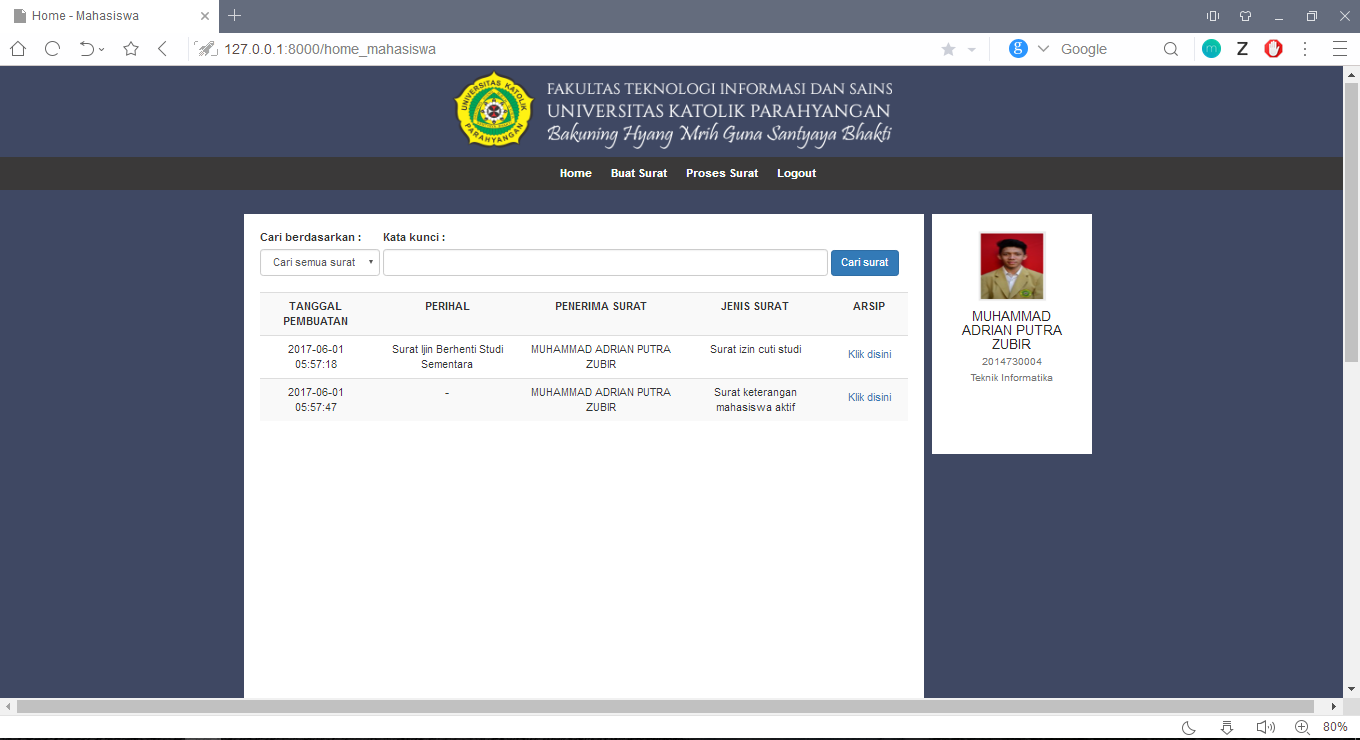
\includegraphics[scale=0.4]{F:/Skripsi/Dokumentasi_Skripsi/Gambar/Ss/Mhs/home_mhs.png}
		\caption{Halaman \textit{home} mahasiswa}
		\label{fig:halaman_home_mahasiswa}
	\end{figure}
	
	\item Halaman pilih kategori surat\\
	Gambar \hyperlink{halaman_pilih_kategori_surat}{5.3} merupakan halaman untuk pemilihan kategori surat apabila mahasiswa menekan menu "Buat Surat" pada \textit{navigation bar}.
	\begin{figure}[H]
	\centering
		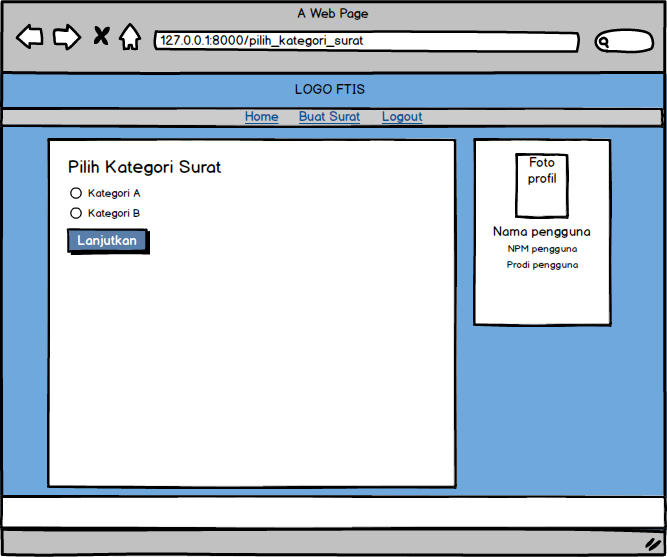
\includegraphics[scale=0.4]{F:/Skripsi/Dokumentasi_Skripsi/Gambar/Ss/Mhs/pilih_kategori_surat.png}
		\caption{Halaman pilih kategori surat}
		\label{fig:halaman_pilih_kategori_surat}
	\end{figure}
	
	 \item Halaman pilih jenis surat\\
	Gambar \hyperlink{halaman_pilih_jenis_surat}{5.4} merupakan halaman untuk pemilihan jenis surat berdasarkan kategori surat yang dipilih sebelumnya.
	\begin{figure}[H]
	\centering
		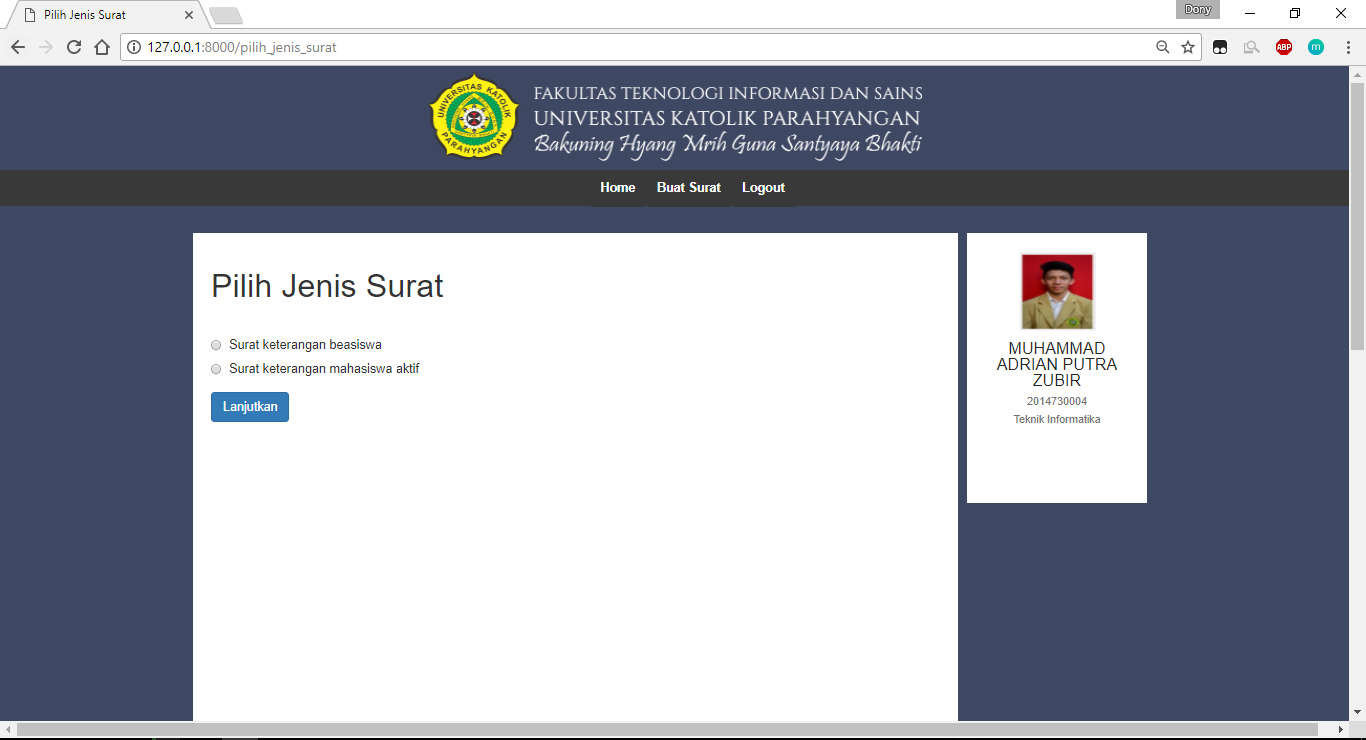
\includegraphics[scale=0.4]{F:/Skripsi/Dokumentasi_Skripsi/Gambar/Ss/Mhs/pilih_jenis_surat.png}
		\caption{Halaman pilih jenis surat}
		\label{fig:halaman_pilih_jenis_surat}
	\end{figure}
	
	\item Halaman pengisian data diri\\
	Gambar \hyperlink{halaman_pengisian_data_diri}{5.5} merupakan halaman pengisian data diri berdasarkan surat yang dipilih oleh mahasiswa.
	\begin{figure}[H]
	\centering
		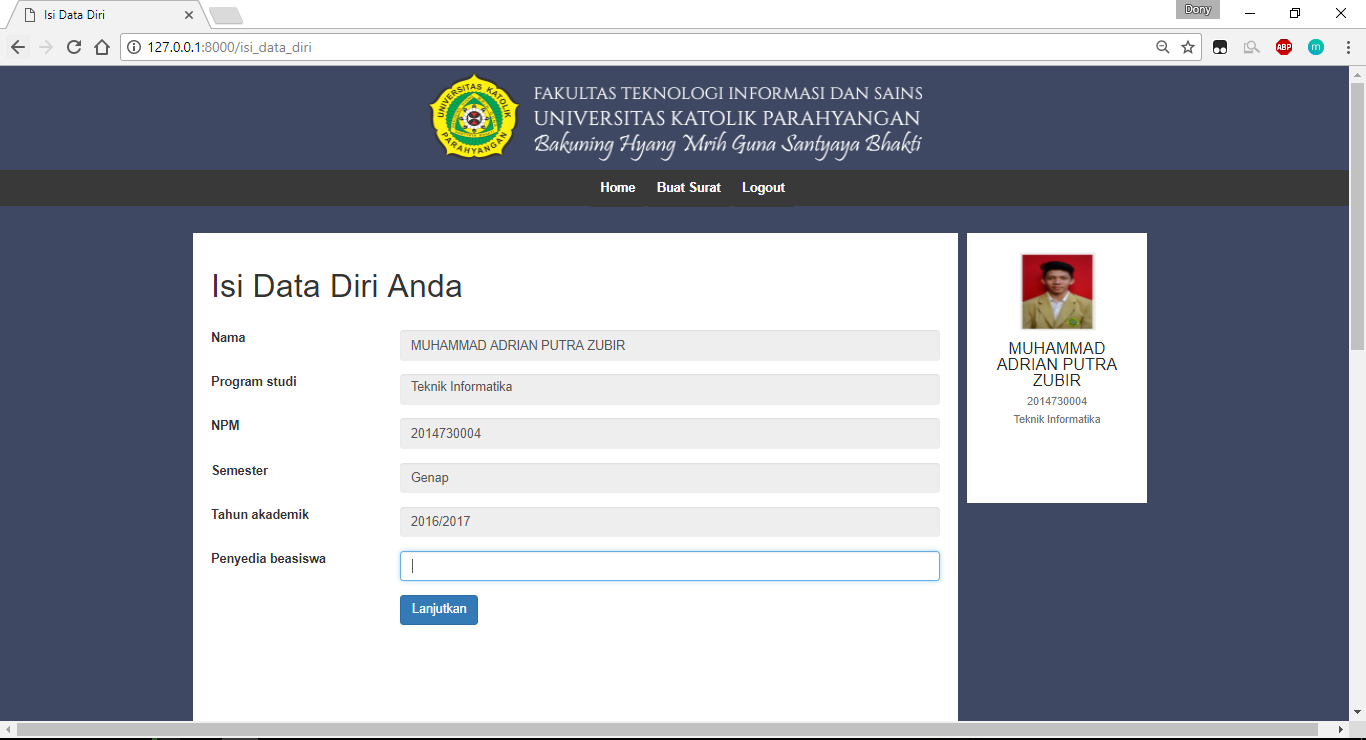
\includegraphics[scale=0.4]{F:/Skripsi/Dokumentasi_Skripsi/Gambar/Ss/Mhs/isi_data_diri.png}
		\caption{Halaman pengisian data diri}
		\label{fig:halaman_pengisian_data_diri}
	\end{figure}
	
	\item Halaman preview\\
	Gambar \hyperlink{halaman_preview_data_diri}{5.6} merupakan halaman untuk melihat data yang telah diisikan pada halaman pengisian data.
	\begin{figure}[H]
	\centering
		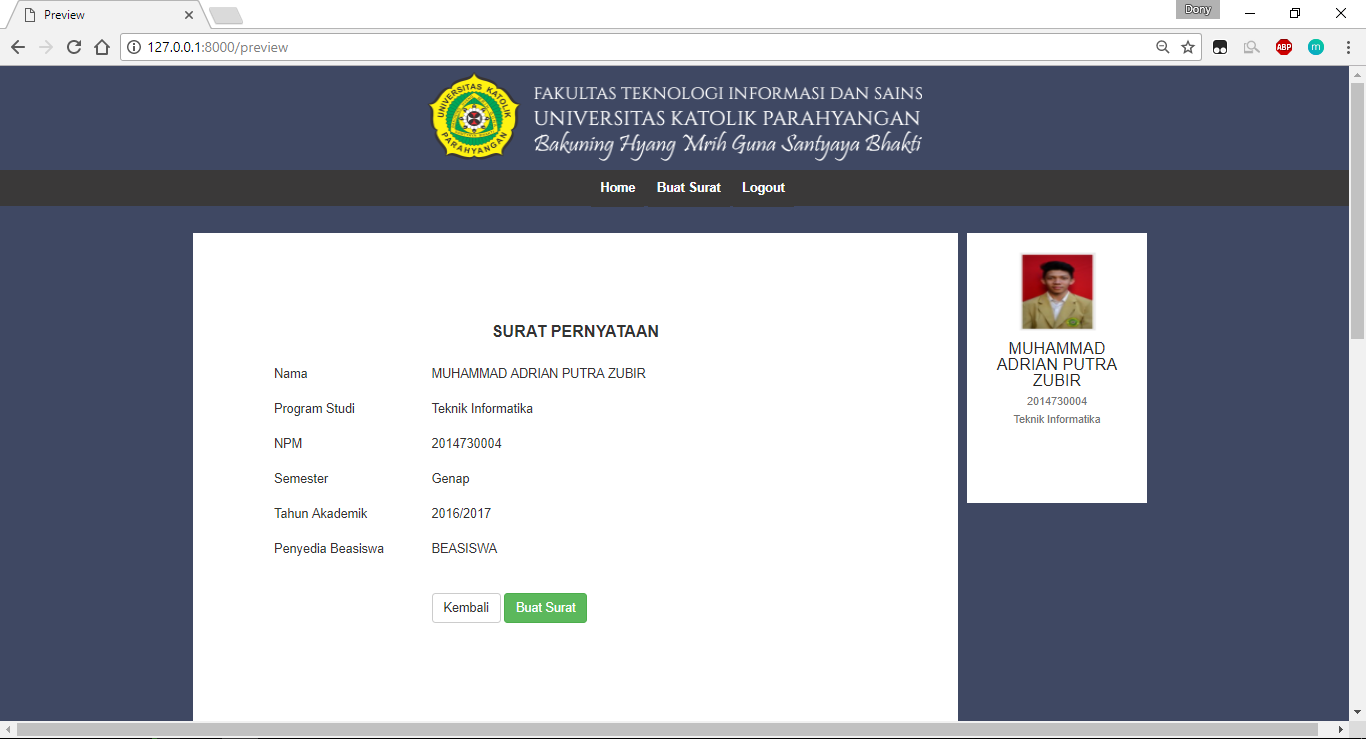
\includegraphics[scale=0.4]{F:/Skripsi/Dokumentasi_Skripsi/Gambar/Ss/Mhs/preview_data_diri.png}
		\caption{Halaman preview data diri}
		\label{fig:halaman_preview_data_diri}
	\end{figure}
\end{itemize}

\subsection{Implementasi Antar Muka Untuk Petugas TU}
\label{sec:implementasi_antar_muka_petugas_tu}
Berdasarkan perancangan antar muka untuk petugas TU, terdapat 8 jenis halaman yang dapat diakses oleh petugas TU. Ketujuh jenis halaman tersebut yaitu :
\begin{itemize}
	\item Halaman \textit{home} tu
	 Gambar \hyperlink{halaman_home_tu}{5.7} merupakan halaman \textit{home} TU yang menampilkan seluruh pesanan surat. Halaman ini merupakan halaman yang pertama kali ditemukan oleh TU setelah berhasil melakukan \textit{login}.
	 \begin{figure}[H]
	\centering
		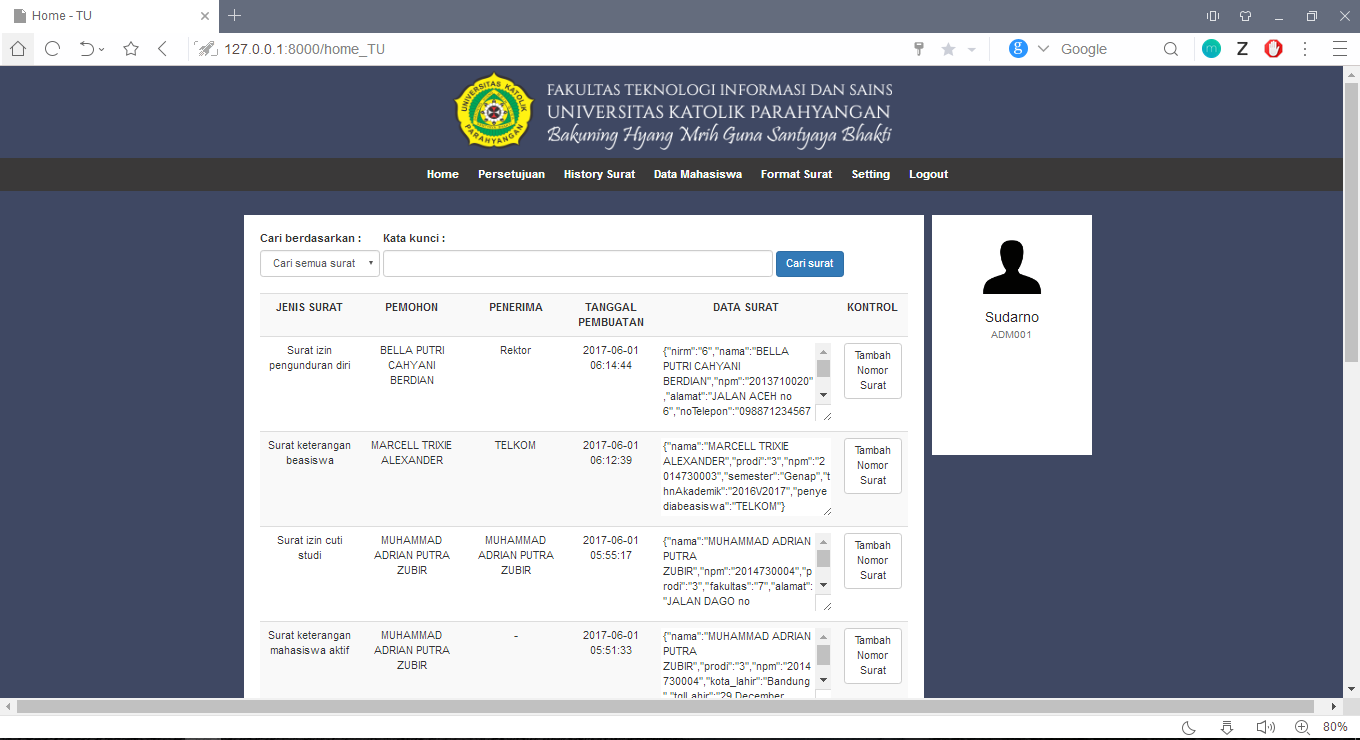
\includegraphics[scale=0.4]{F:/Skripsi/Dokumentasi_Skripsi/Gambar/Ss/TU/home_tu.png}
		\caption{Halaman \textit{home} TU}
		\label{fig:halaman_home_tu}
	\end{figure}

	\item Halaman data mahasiswa\\
	 Gambar \hyperlink{implementasi_halaman_data_mahasiswa}{5.8} merupakan halaman data mahasiswa yang menampilkan seluruh mahasiswa yang terdaftar.
	 \begin{figure}[H]
	\centering
		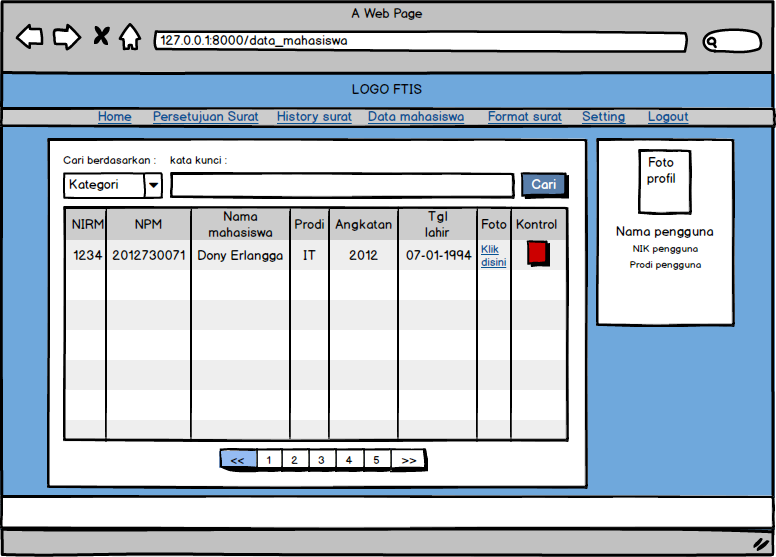
\includegraphics[scale=0.4]{F:/Skripsi/Dokumentasi_Skripsi/Gambar/Ss/TU/data_mahasiswa.png}
		\caption{Halaman data mahasiswa}
		\label{fig:implementasi_halaman_data_mahasiswa}
	\end{figure}
	
	\item Halaman format surat\\
	 Gambar \hyperlink{implementasi_halaman_format_surat}{5.9} merupakan halaman format surat yang menampilkan seluruh format surat yang tersedia.
	 \begin{figure}[H]
	\centering
		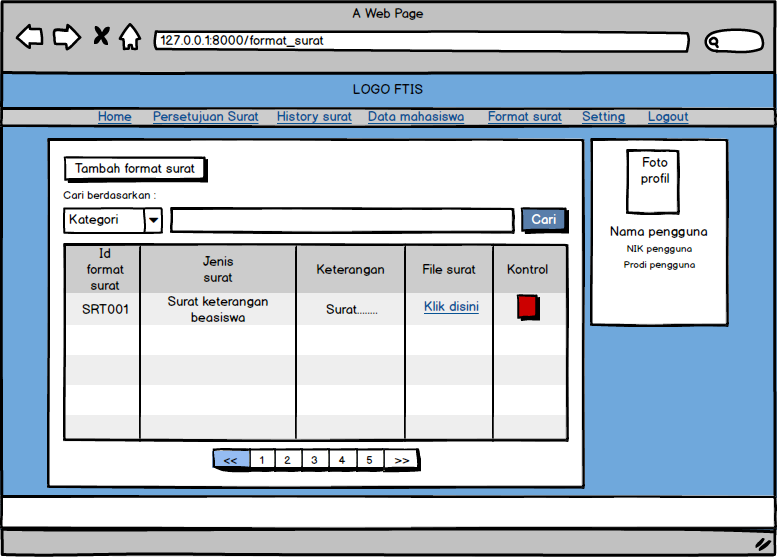
\includegraphics[scale=0.4]{F:/Skripsi/Dokumentasi_Skripsi/Gambar/Ss/TU/format_surat.png}
		\caption{Halaman format surat}
		\label{fig:implementasi_halaman_format_surat}
	\end{figure}
	
	\item Halaman \textit{home} mahasiswa\\
	 Gambar \hyperlink{implementasi_halaman_tambah_format_surat}{5.10} merupakan halaman untuk menambahkan format surat baru.
	 \begin{figure}[H]
	\centering
		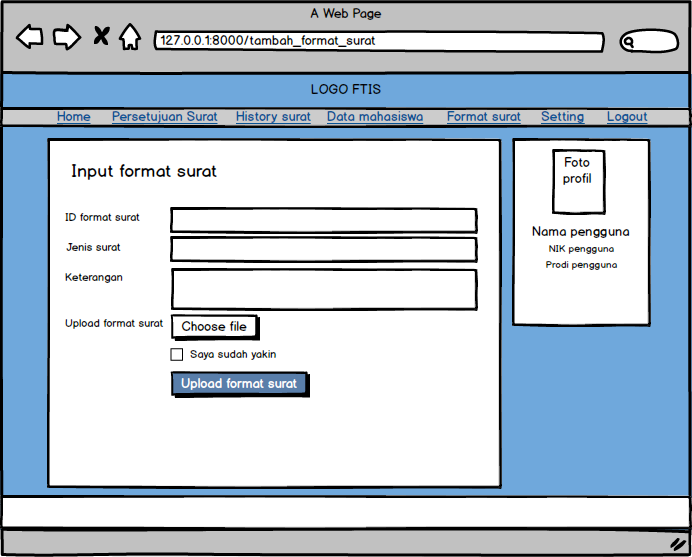
\includegraphics[scale=0.4]{F:/Skripsi/Dokumentasi_Skripsi/Gambar/Ss/TU/tambah_format_surat.png}
		\caption{Halaman tambah format surat}
		\label{fig:implementasi_halaman_tambah_format_surat}
	\end{figure}
	
	\item Halaman \textit{history} surat\\
	 Gambar \hyperlink{halaman_history_tu}{5.11} merupakan halaman \textit{history} surat yang menampilkan seluruh \textit{history} dari surat yang pernah dibuat.
	 \begin{figure}[H]
	\centering
		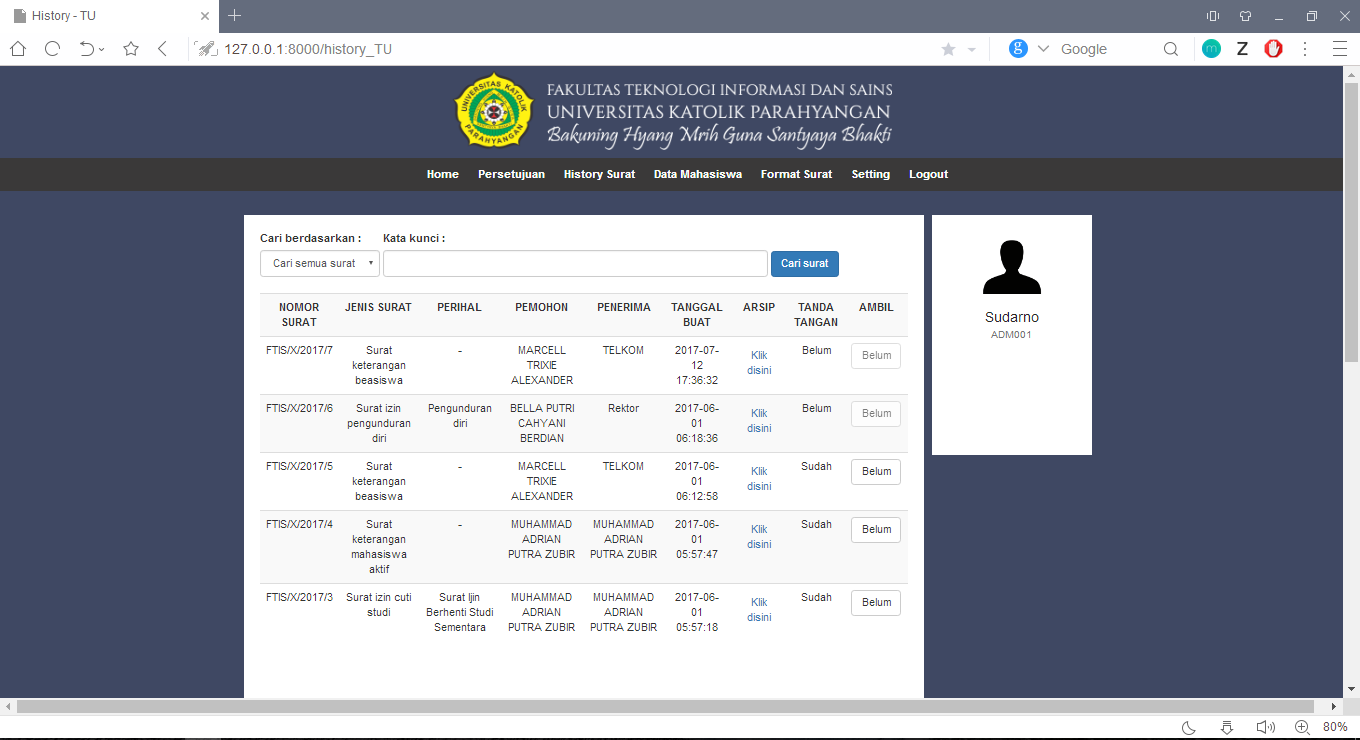
\includegraphics[scale=0.4]{F:/Skripsi/Dokumentasi_Skripsi/Gambar/Ss/TU/history_tu.png}
		\caption{Halaman \textit{history} TU}
		\label{fig:halaman_history_tu}
	\end{figure}
	
	\item Halaman tambah nomor surat\\
	 Gambar \hyperlink{halaman_tambah_nomor_surat}{5.12} merupakan halaman untuk menambahkan nomor surat. Apabila nomor surat sudah diisikan, dapat menekan tombol buat surat untuk meng-\textit{generate} surat dalam bentuk \textit{file} PDF.
	 \begin{figure}[H]
	\centering
		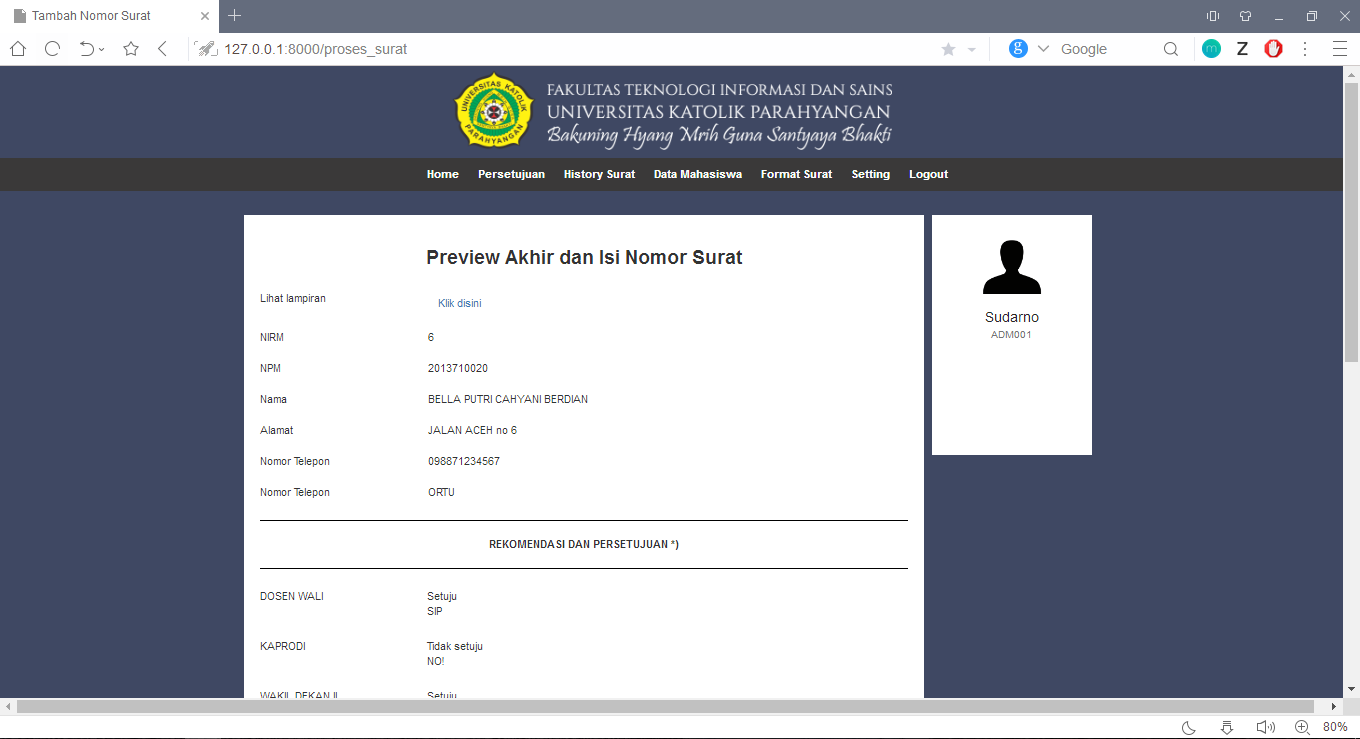
\includegraphics[scale=0.4]{F:/Skripsi/Dokumentasi_Skripsi/Gambar/Ss/TU/tambah_noSurat.png}
		\caption{Halaman tambah nomor surat}
		\label{fig:halaman_tambah_nomor_surat}
	\end{figure}
	
	\item Halaman \textit{setting} semseter dan tahun akademik terkini\\
	 Gambar \hyperlink{halaman_setting_semester_dan_tahun_akademik_terkini}{5.13} merupakan halaman untuk mengubah semester dan tahun akademik yang berlaku untuk pada suatu semester.
	 \begin{figure}[H]
	\centering
		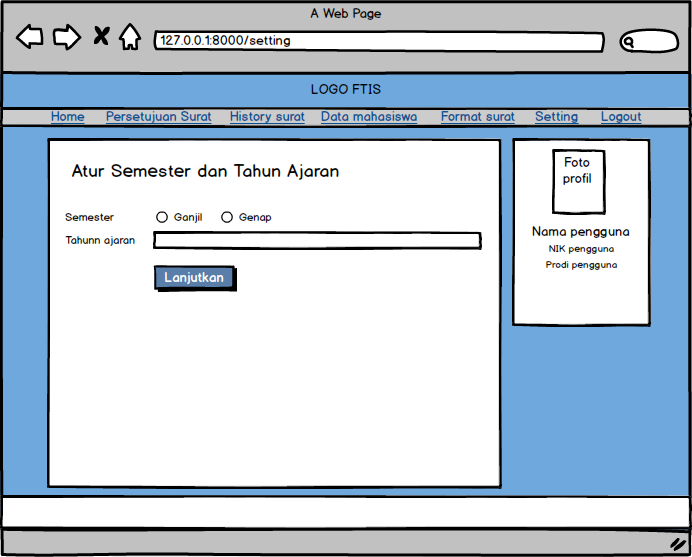
\includegraphics[scale=0.4]{F:/Skripsi/Dokumentasi_Skripsi/Gambar/Ss/TU/setting.png}
		\caption{Halaman \textit{setting} semester dan tahun akademik terkini}
		\label{fig:halaman_setting_semester_dan_tahun_akademik_terkini}
	\end{figure}
	
	\item Halaman persetujuan pejabat\\
	 Gambar \hyperlink{halaman_persetujuan_pejabat}{5.14} merupakan halaman untuk memantau proses persetujuan surat yang dipesan oleh seluruh mahasiswa.
	 \begin{figure}[H]
	\centering
		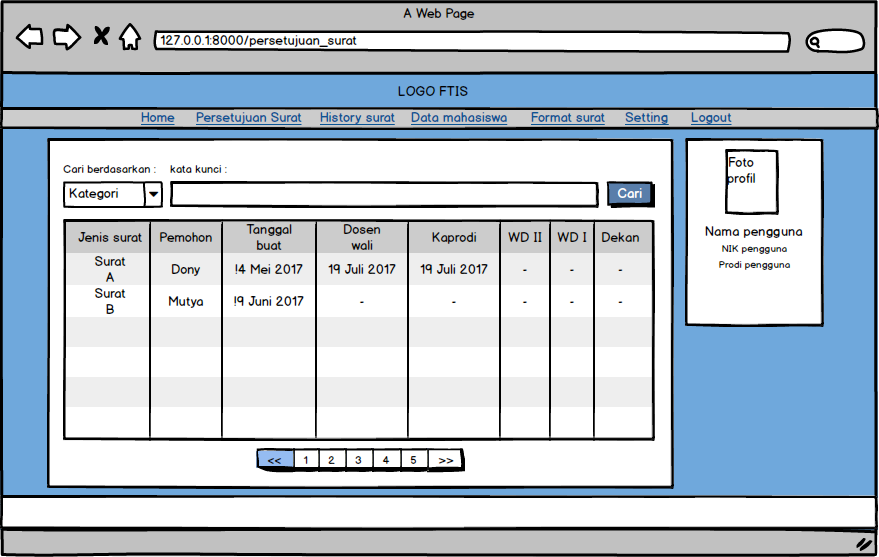
\includegraphics[scale=0.4]{F:/Skripsi/Dokumentasi_Skripsi/Gambar/Ss/TU/persetujuan_surat.png}
		\caption{Halaman persetujuan surat}
		\label{fig:halaman_persetujuan_pejabat}
	\end{figure}
\end{itemize}
	
\subsection{Implementasi Antar Muka Untuk Pejabat}
\label{sec:implementasi_antar_muka_pejabat}
Berdasarkan perancangan antar muka untuk pejabat, terdapat 4 jenis halaman yang dapat diakses oleh pejabat. Keempat jenis halaman tersebut yaitu :
\begin{itemize}
	\item Halaman \textit{home} pejabat\\
	 Gambar \hyperlink{halaman_home_pejabat}{5.15} merupakan halaman \textit{home} pejabat yang menampilkan seluruh pesanan surat. Halaman ini merupakan halaman yang pertama kali ditemukan oleh pejabat setelah berhasil melakukan \textit{login}.
	 \begin{figure}[H]
	\centering
		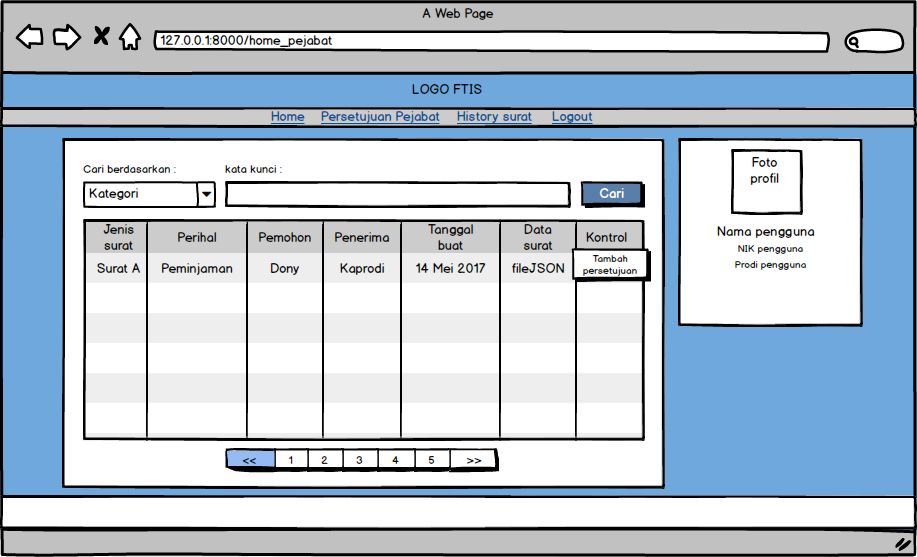
\includegraphics[scale=0.4]{F:/Skripsi/Dokumentasi_Skripsi/Gambar/Ss/Pejabat/home_pejabat.png}
		\caption{Halaman \textit{home} pejabat}
		\label{fig:halaman_home_pejabat}
	\end{figure}
	
	\item Halaman pengisian persetujuan dan catatan\\
	 Gambar \hyperlink{halaman_persetujuan_dan_catatan}{5.16} merupakan halaman pengisian persetujuan dan catatan untuk jenis surat izin cuti studi dan surat izin pengunduran diri.
	 \begin{figure}[H]
	\centering
		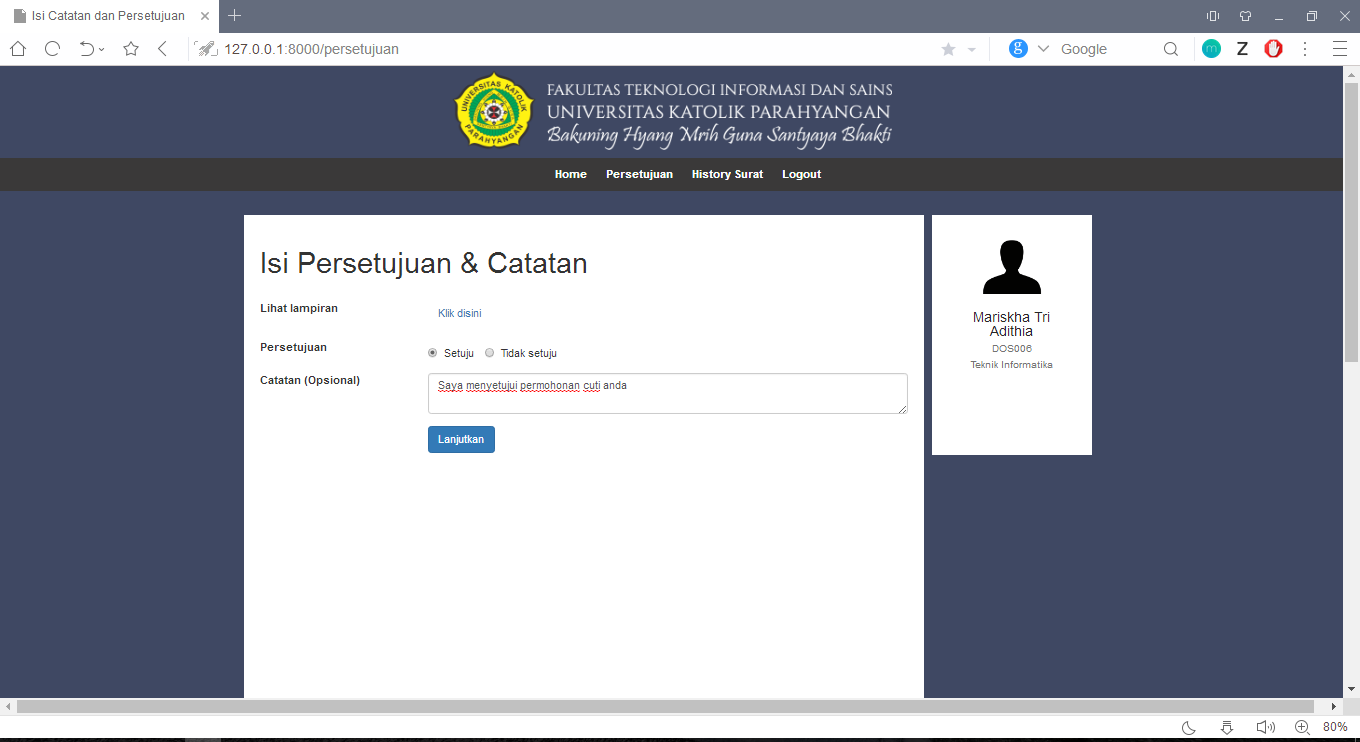
\includegraphics[scale=0.4]{F:/Skripsi/Dokumentasi_Skripsi/Gambar/Ss/Pejabat/tambah_persetujuan.png}
		\caption{Halaman pengisian persetujuan dan catatan}
		\label{fig:halaman_persetujuan_dan_catatan}
	\end{figure}
	
	\item Halaman \textit{preview} pengisian persetujuan dan catatan\\
	 Gambar \hyperlink{halaman_preview_persetujuan_dan_catatan}{5.17} merupakan halaman \textit{preview} pengisian persetujuan dan catatan untuk jenis surat izin cuti studi dan surat izin pengunduran diri.
	 \begin{figure}[H]
	\centering
		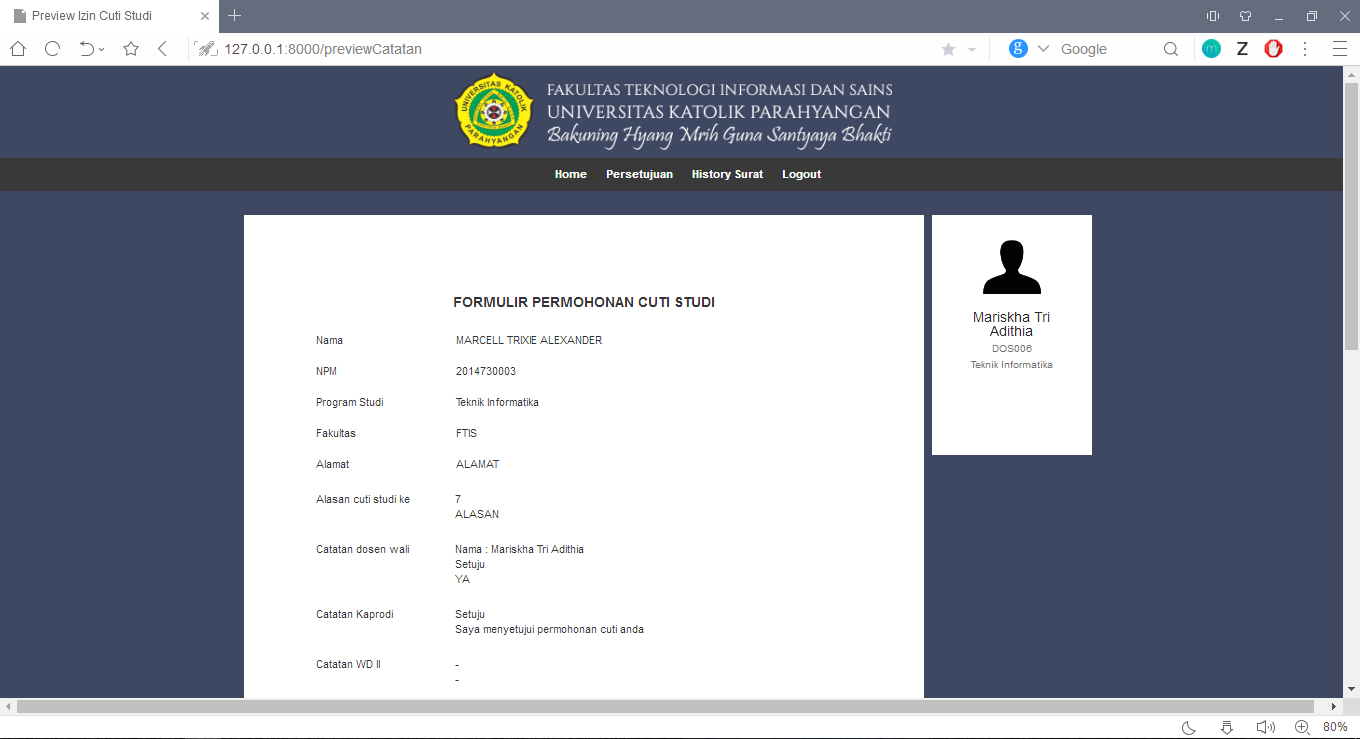
\includegraphics[scale=0.4]{F:/Skripsi/Dokumentasi_Skripsi/Gambar/Ss/Pejabat/preview_pejabat.png}
		\caption{Halaman \textit{preview} pengisian persetujuan dan catatan}
		\label{fig:halaman_preview_persetujuan_dan_catatan}
	\end{figure}
	
	\item Halaman persetujuan pejabat\\
	 Gambar \hyperlink{halaman_persetujuan_surat}{5.18} merupakan halaman untuk memantau proses persetujuan surat yang dipesan oleh mahasiswa yang menjadi anak bimbing dari dosen yang melakukan \textit{login} saja.
	 \begin{figure}[H]
	\centering
		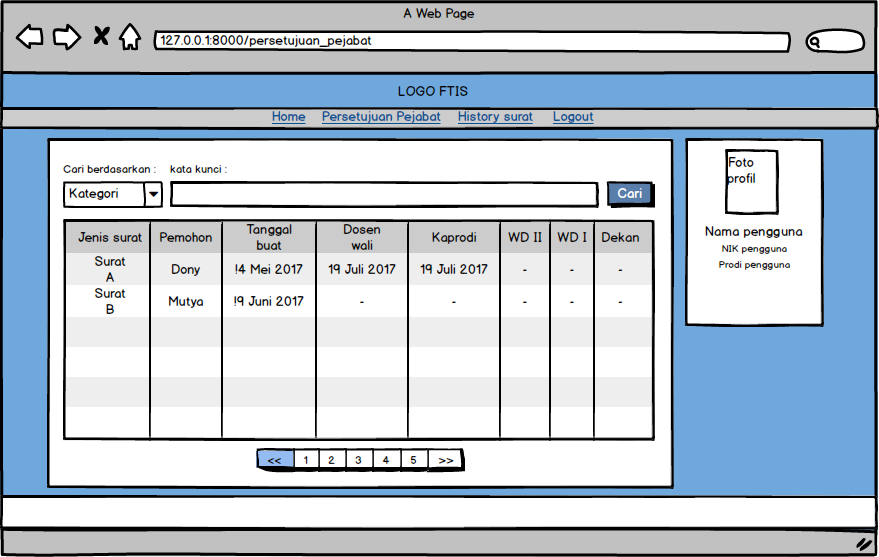
\includegraphics[scale=0.4]{F:/Skripsi/Dokumentasi_Skripsi/Gambar/Ss/Pejabat/persetujuan_pejabat.png}
		\caption{Halaman persetujuan surat}
		\label{fig:halaman_persetujuan_surat}
	\end{figure}
\end{itemize}

\section{Implementasi Kode Program Untuk \textit{Compile File} Surat}
\label{sec:implementasi_kode_program_untuk_compile_file_surat}
Untuk meng-\textit{compile} \textit{file} surat dari format \textit{.tex} ke format \textit{.pdf}, digunakan fungsi yang terdapat pada \textit{file} HistorysuratController.php berikut ini.
\begin{lstlisting}[language=php, basicstyle=\tiny, caption=Fungsi untuk meng-\textit{compile} surat]
	if($request->idFormatSurat == "1"){
        $dataSurat = $request->data;
        $json = json_decode($dataSurat);
        $noSurat = $request->noSurat;
        $nama = $json->nama;
        $prodi = $this->jurusanRepo->findJurusanById($json->prodi)->nama_jurusan;
        $npm = $json->npm;
        $semester = $json->semester;
        $thnAkademik = $json->thnAkademik;
        $penyediabeasiswa = $json->penyediabeasiswa;
        $pemesan = $request->pemesan;
        
        $getLocal = getdate();
        $toString = implode(" ", $getLocal);
        $getDate = explode(" ",$toString);
        $arrTanggal = $getDate[6].'-'.$getDate[5].'-'.$getDate[3];
        $getTanggal = date_create($arrTanggal);
        $tanggal = $getTanggal->format("j F Y");

        $entry = '\mailentry{' . $noSurat . ',' . $nama . ',' . $prodi . ',' . $npm . ',' . $semester . ',' . $thnAkademik . ',' . $penyediabeasiswa . ',' . $tanggal . '}';
        $fileTemplate = file('format_surat_latex/surat_keterangan_beasiswa.tex');
        $stringFormat = "";
        $baris = count($fileTemplate);

        foreach ($fileTemplate as $line_num => $line) {
            $stringFormat .= $line;
            if($line_num == $baris-3){
                $stringFormat .= $entry;
            }
        }

        $file = fopen("arsip_surat/" . $npm . "_surat_keterangan_beasiswa.tex", "w");
        fwrite($file, $stringFormat);
        fclose($file);
        shell_exec('pdflatex -output-directory arsip_surat arsip_surat/' . $npm . '_surat_keterangan_beasiswa.tex');

        $historysurat = new Historysurat;
        $historysurat->no_surat = $noSurat;
        $historysurat->perihal = '-';
        $historysurat->penerimaSurat = $json->penyediabeasiswa;
        $historysurat->mahasiswa_id = $pemesan;
        $historysurat->formatsurat_id = $request->idFormatSurat;
        $historysurat->link_arsip_surat = 'arsip_surat/' . $npm . '_surat_keterangan_beasiswa.pdf';
        $historysurat->penandatanganan = false;
        $historysurat->pengambilan = false;
        $historysurat->save();
        return redirect('/history_TU');
      }
\end{lstlisting}

\section{Pengujian}
\label{sec:pengujian}
Bagian ini membahas mengenai pengujian fitur yang dilakukan pada \textit{website} SIKSA. Metode pengujian yang digunakan yaitu metode \textit{black box testing}, yaitu metode pengujian perangkat lunak dengan mencoba sebanyak mungkin contoh kasus ke dalam sistem tanpa melihat kode program untuk menemukan kesalahan.
\begin{itemize}
	\item Pengujian \textit{login}
	\begin{table}[H]
	\centering
	\caption{Tabel pengujian \textit{login}}
	\label{pengujian_login}
	\begin{tabular}{|l|p{6cm}|p{6cm}|}
	\hline
	\textbf{No.}&\textbf{Langkah Pengujian}&\textbf{Hasil yang Diharapkan}\\ \hline
	1&Pengguna memasukkan \textit{username} dan \textit{password} dengan benar&Pengguna berhasil masuk ke halaman \textit{home} yang sesuai dengan \textit{role}-nya \\ \hline
	2&Pengguna memasukkan \textit{username} atau \textit{password} yang salah &Pengguna akan kembali ke halaman login dan sistem mengembalikan pesan \textit{error}\\ \hline
	3&Pengguna hanya memasukkan salah satu dari \textit{username} atau \textit{password}&Pengguna akan diminta untuk mengisi bagian yang belum diisi\\ \hline
	4&Pengguna tidak memasukkan \textit{username} dan \textit{password}p{6cm}|p{6cm}&Pengguna akan diminta untuk mengisi \textit{username} dan \textit{password}\\ \hline
	\end{tabular}
	\end{table}	
	
	\item Pengujian pembuatan surat oleh mahasiswa
	\begin{table}[H]
	\centering
	\caption{Tabel pengujian pembuatan surat oleh mahasiswa}
	\label{pengujian_pembuatan_surat_oleh_mahasiswa}
	\begin{tabular}{|l|p{6cm}|p{6cm}|}
	\hline
	\textbf{No.}&\textbf{Langkah Pengujian}&\textbf{Hasil yang Diharapkan}\\ \hline
	1&Mahasiswa membuat surat keterangan beasiswa&Mahasiswa mendapatkan surat keterangan beasiswa yang sudah siap dicetak\\ \hline
	2&Mahasiswa membuat surat keterangan mahasiswa aktif&Mahasiswa mendapatkan surat keterangan mahasiswa aktif yang sudah siap dicetak\\ \hline
	3&Mahasiswa membuat surat pengantar pembuatan visa&Mahasiswa mendapatkan surat pengantar pembuatan visa yang sudah siap dicetak\\ \hline
	4&Mahasiswa membuat surat pengantar studi lapangan perorangan &Mahasiswa mendapatkan surat pengantar studi lapangan perorangan yang sudah siap dicetak\\ \hline
	5&Mahasiswa membuat surat pengantar studi lapangan untuk 2 orang &Mahasiswa mendapatkan surat pengantar studi lapangan untuk 2 orang yang sudah siap dicetak\\ \hline
	6&Mahasiswa membuat surat pengantar studi lapangan untuk 3 orang &Mahasiswa mendapatkan surat pengantar studi lapangan untuk 3 orang yang sudah siap dicetak\\ \hline
	7&Mahasiswa membuat surat pengantar studi lapangan untuk 4 orang &Mahasiswa mendapatkan surat pengantar studi lapangan untuk 4 orang yang sudah siap dicetak\\ \hline
	8&Mahasiswa membuat surat pengantar studi lapangan untuk 5 orang &Mahasiswa mendapatkan surat pengantar studi lapangan untuk 5 orang yang sudah siap dicetak\\ \hline
	9&Mahasiswa membuat surat izin cuti studi&Mahasiswa mendapatkan surat izin cuti studi yang sudah siap dicetak\\ \hline
	10&Mahasiswa membuat surat izin pengunduran diri&Mahasiswa mendapatkan surat pengunduran diri yang sudah siap dicetak\\ \hline
	\end{tabular}
	\end{table}	
	
	\begin{table}[H]
	\centering
	\begin{tabular}{|l|p{6cm}|p{6cm}|}
	\hline
	11&Mahasiswa membuat surat perwakilan perwalian untuk pengambilan 1 mata kuliah&Mahasiswa mendapatkan surat perwakilan perwalian untuk pengambilan 1 mata kuliah yang sudah siap dicetak\\ \hline
	12&Mahasiswa membuat surat perwakilan perwalian untuk pengambilan 2 mata kuliah&Mahasiswa mendapatkan surat perwakilan perwalian untuk pengambilan 2 mata kuliah yang sudah siap dicetak\\ \hline
	13&Mahasiswa membuat surat perwakilan perwalian untuk pengambilan 3 mata kuliah&Mahasiswa mendapatkan surat perwakilan perwalian untuk pengambilan 3 mata kuliah yang sudah siap dicetak\\ \hline
	14&Mahasiswa membuat surat perwakilan perwalian untuk pengambilan 4 mata kuliah&Mahasiswa mendapatkan surat perwakilan perwalian untuk pengambilan 4 mata kuliah yang sudah siap dicetak\\ \hline
	15&Mahasiswa membuat surat perwakilan perwalian untuk pengambilan 5 mata kuliah&Mahasiswa mendapatkan surat perwakilan perwalian untuk pengambilan 5 mata kuliah yang sudah siap dicetak\\ \hline
	16&Mahasiswa membuat surat perwakilan perwalian untuk pengambilan 6 mata kuliah&Mahasiswa mendapatkan surat perwakilan perwalian untuk pengambilan 6 mata kuliah yang sudah siap dicetak\\ \hline
	17&Mahasiswa membuat surat perwakilan perwalian untuk pengambilan 7 mata kuliah&Mahasiswa mendapatkan surat perwakilan perwalian untuk pengambilan 7 mata kuliah yang sudah siap dicetak\\ \hline
	18&Mahasiswa membuat surat perwakilan perwalian untuk pengambilan 8 mata kuliah&Mahasiswa mendapatkan surat perwakilan perwalian untuk pengambilan 8 mata kuliah yang sudah siap dicetak\\ \hline
	19&Mahasiswa membuat surat perwakilan perwalian untuk pengambilan 9 mata kuliah&Mahasiswa mendapatkan surat perwakilan perwalian untuk pengambilan 9 mata kuliah yang sudah siap dicetak\\ \hline
	20&Mahasiswa membuat surat perwakilan perwalian untuk pengambilan 10 mata kuliah&Mahasiswa mendapatkan surat perwakilan perwalian untuk pengambilan 10 mata kuliah yang sudah siap dicetak\\ \hline
	\end{tabular}
	\end{table}	
	
	\item Pengujian memberikan nomor surat dan \textit{generate} surat
	\begin{table}[H]
	\centering
	\caption{Tabel pengujian memberikan nomor surat dan \textit{generate} surat}
	\label{pengujian_memberikan_nomor_surat_dan_generate_surat}
	\begin{tabular}{|l|p{6cm}|p{6cm}|}
	\hline
	\textbf{No.}&\textbf{Langkah Pengujian}&\textbf{Hasil yang Diharapkan}\\ \hline
	1&Petugas TU menambahkan nomor surat&Surat bernomor\\ \hline
	\end{tabular}
	\end{table}
	
	\item Pengujian mengubah status penandatanganan surat
	\begin{table}[H]
	\centering
	\caption{Tabel pengujian mengubah status penandatanganan surat}
	\label{pengujian_mengubah_status_penandatanganan_surat}
	\begin{tabular}{|l|p{6cm}|p{6cm}|}
	\hline
	\textbf{No.}&\textbf{Langkah Pengujian}&\textbf{Hasil yang Diharapkan}\\ \hline
	1&Petugas TU menekan tombol untuk mengubah status penandatanganan surat&Status penandatanganan surat berubah menjadi "`Sudah"' \\ \hline
	\end{tabular}
	\end{table}
	
	\item Pengujian mengubah status pengambilan surat
	\begin{table}[H]
	\centering
	\caption{Tabel pengujian mengubah status pengambilan surat}
	\label{pengujian_mengubah_status_pengambilan_surat}
	\begin{tabular}{|l|p{6cm}|p{6cm}|}
	\hline
	\textbf{No.}&\textbf{Langkah Pengujian}&\textbf{Hasil yang Diharapkan}\\ \hline
	1&Petugas TU menekan tombol untuk mengubah status pengambilan surat setelah status penandatanganan surat menjadi "`Sudah"'&Status pengambilan berubah menjadi sudah \\ \hline
	2&Petugas TU menekan tombol untuk mengubah status pengambilan surat saat status penandatanganan surat masih"`Belum"'&Tombol untuk mengubah status pengambilan surat tidak bisa ditekan\\ \hline
	\end{tabular}
	\end{table} 
	
	\item Pengujian menghapus mahasiswa
	\begin{table}[H]
	\centering
	\caption{Tabel pengujian menghapus mahasiswa}
	\label{pengujian_menghapus_mahasiswa}
	\begin{tabular}{|l|p{6cm}|p{6cm}|}
	\hline
	\textbf{No.}&\textbf{Langkah Pengujian}&\textbf{Hasil yang Diharapkan}\\ \hline
	1&Petugas TU menekan tombol untuk menghapus mahasiswa&Mahasiswa terhapus \\ \hline
	\end{tabular}
	\end{table}
	
	\item Pengujian menghapus format surat
	\begin{table}[H]
	\centering
	\caption{Tabel pengujian menghapus format surat}
	\label{pengujian_menghapus_format_surat}
	\begin{tabular}{|l|p{6cm}|p{6cm}|}
	\hline
	\textbf{No.}&\textbf{Langkah Pengujian}&\textbf{Hasil yang Diharapkan}\\ \hline
	1&Petugas TU menekan tombol untuk menghapus format surat&Format surat terhapus\\ \hline
	\end{tabular}
	\end{table}
	
	\item Pengujian menambah format surat
	\begin{table}[H]
	\centering
	\caption{Tabel pengujian menambah format surat}
	\label{pengujian_menambah_format_surat}
	\begin{tabular}{|l|p{6cm}|p{6cm}|}
	\hline
	\textbf{No.}&\textbf{Langkah Pengujian}&\textbf{Hasil yang Diharapkan}\\ \hline
	1&Petugas TU menambahkan format surat baru beserta idFormatSurat, jenis surat beserta keterangan&Format surat tersimpan di \textit{database}\\ \hline
	\end{tabular}
	\end{table}
	
	\item Pengujian mengubah semester dan tahun akademik pada setiap data mahasiswa yang terdaftar
	\begin{table}[H]
	\centering
	\caption{Tabel pengujian mengubah semester dan tahun akademik pada setiap data mahasiswa yang terdaftar}
	\label{pengujian_mengubah_semester_dan_tahun_akademik}
	\begin{tabular}{|l|p{6cm}|p{6cm}|}
	\hline
	\textbf{No.}&\textbf{Langkah Pengujian}&\textbf{Hasil yang Diharapkan}\\ \hline
	1&Petugas TU mengubah semester dan tahun akademik&\textit{Field} semester dan tahun ajaran pada tabel mahasiswa berubah sesuai dengan semester dan tahun ajaran yang dimasukkan\\ \hline
	\end{tabular}
	\end{table}
	
\end{itemize}